% 几何矢量
% 线性代数|几何矢量|代数矢量|单位矢量|标量|平行四边形法则|线性组合|线性相关|线性无关|基底|矢量空间|坐标

\pentry{集合\upref{Set}, 充分必要条件\upref{SufCnd}}

我们来回顾高中学的\textbf{几何矢量}, 本文中简称为“矢量”. 矢量是空间中的一些有长度有方向的箭头. 我们对它的位置不感兴趣, 所有长度和方向相同的矢量都视为同一矢量. 本书中矢量用正黑体表示, 如 $\bvec a$. 在手写时, 可以在字母上方加箭头表示, 如 $\overrightarrow{a}$. 特殊地, 如果一个矢量的长度等于 1, 那么它就是一个\textbf{单位矢量}, 本书中在矢量上面加上 “\^{}” 符号表示单位矢量, 如 $\uvec a$. 为了与矢量区分, 我们把单个的实数或复数称为\textbf{标量}.

\subsection{几何矢量}

\textbf{矢量(vector)}又被翻译为\textbf{向量}.这个概念最初来自直观的几何矢量.早在民国时期,学者们引入vector的概念时就将它译成了汉语. 由于当时的物理学家和数学家没有太多交集, 物理学家将它翻译为向量, 而数学家翻译为矢量. 90 年代时, 国家名词委员会商议确定一个统一的 vector 译名, 但却无法轻易割舍两个译名中的任何一个, 因为它们都非常信达雅地表明了vector 的含义:向量即有方向的量, 矢量即像箭矢一样的量. 大概是出自物理学家和数学家的互相尊重, 最后确定的方案是双方互换译名, 从此物理学界称矢量, 数学界称矢量\footnote{以下加粗部分为力学家朱照宣教授的回忆.\textbf{在20世纪90年代初,国家名词委为此(vector)召开会议,想协调双方,由主任钱三强亲自主持. 我曾戏称这是个 “一字会”. 当时的情况是, 学科有分支, 术语有派生, 犹如家族有后裔. 祖宗互相谦让, 但子孙繁多, 已无法协调. 钱先生在会上没有说倾向于哪方面的话. 矢量、向量的分歧,一直维持到今. 力学这学科, 和数学、物理同样有 “亲”, 力学中 vector 用什么? 当年我在 “一字会” 后还有情绪, 埋怨钱先生作为领导“不表态”. 过了好些年,才懂得这类事,最多只能因势利导, 不能靠行政命令或专家拍板. 事实上, 台湾物理界至今用的是还 “向量”.}}. 本书中不区分两个译名的使用.

本词条中讨论的\textbf{几何矢量}, 也是经典物理学中最长见的一类矢量, 是一种具有\textbf{长度}和\textbf{方向}的量,因此可以画成箭头来表示.生活中这样具有长度和方向的量十分常见: 速度有大小有方向,因此可以表示为箭头,箭头的长度代表速度的大小;加速度\upref{VnA}也有大小, 有方向; 我从一个地方运动到另一个地方,那么从起点到终点可以画一根箭头, 这箭头就是位移矢量\upref{Disp}. 不止在生活中, 一切领域里具有方向和大小概念的量都被称为几何矢量. 不过,在数学中,矢量的含义要比几何矢量更广泛,也就是说,几何矢量是数学家所研究的矢量的一种, 但不是唯一的一种. 作为一个预热, 在线性代数中, 我们把这些最为直观的几何矢量构成的集合,称作 “实数域上的赋范线性空间”.

特别地,长度为零的矢量称为\textbf{零矢量(zero vector)}, 不作方向区分(可以认为它与任何矢量平行). 零矢量依然是矢量, 要注意和数字零进行区分.

几何矢量本身可以单独存在,而不需要借助任何坐标系或坐标来描述.事实上,随着坐标系的不同,一个矢量的坐标也往往不同.下面要介绍的许多概念(加法, 数乘, 线性组合, 线性无关等)都不需要任何坐标的概念,请试着摆脱具体的坐标来理解它们.

\subsection{几何矢量的运算}

把所有几何矢量收集到一起,构成一个集合,本身没什么可以研究的.在集合\upref{Set}中我们说过,没有任何附加结构的集合中,元素叫什么都不重要,只有元素数量重要.为了让矢量集合有讨论的意义,我们引入了矢量的运算,这样,矢量集合就有了运算结构.

\subsubsection{矢量的加法}
第一个矢量运算,是矢量间的加法.两个矢量相加,结果是另一个矢量,其定义如下.

如\autoref{GVec_fig1},两个矢量相加, 既可以使用平行四边形法则, 也可以用三角形法则. 若有多个矢量连续相加, 可以分别把它们首尾相接, 结果就是由起点指向终点的矢量. 容易证明矢量的加法满足加法交换律 $\bvec A + \bvec B = \bvec B + \bvec A$, 结合律 $(\bvec A + \bvec B) + \bvec C = \bvec A + (\bvec B + \bvec C)$.
\begin{figure}[ht]
\centering
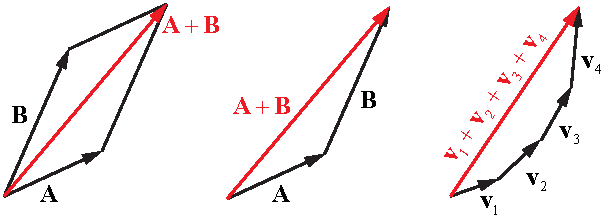
\includegraphics[width=10.5cm]{./figures/GVec_1.pdf}
\caption{矢量的加法} \label{GVec_fig1}
\end{figure}
再次强调无论如何平移一个矢量, 我们都将它看成是同一个矢量.

\subsubsection{矢量的数乘\ 共线}
第二个矢量运算,是一个矢量和一个数字的乘积,得到一个矢量,称为数乘,我们用例子定义如下.

如\autoref{GVec_fig2}, 一个矢量与一个正实数相乘, 则方向不变, 把长度乘以这个实数. 若这个数是负数, 则把矢量取反方向再把长度乘以这个实数数的绝对值即可.若 $\lambda, \mu$ 表示实数, 容易证明分配律 $\lambda(\bvec A + \bvec B) = \lambda\bvec A + \lambda\bvec B$ 和 $(\lambda+\mu)\bvec A = \lambda\bvec A + \mu\bvec A$, 结合律 $\lambda(\mu\bvec A) = (\lambda\mu) \bvec A$.
\begin{figure}[ht]
\centering
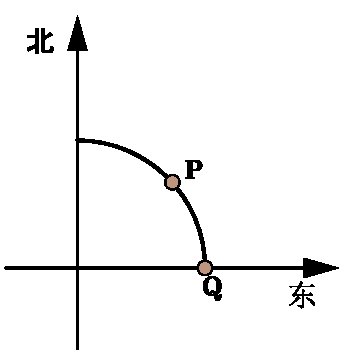
\includegraphics[width=6.5cm]{./figures/GVec_2.pdf}
\caption{矢量的数乘} \label{GVec_fig2}
\end{figure}

如果两个矢量的关系可以用 $\bvec A = \lambda\bvec B$ 表示, 那么它们就是\textbf{共线}的. 共线的充分必要条件\upref{SufCnd}是, 两矢量方向相同或相反.

\subsubsection{矢量的线性组合}
把有限个矢量 $\bvec v_i$ 分别与若干实数 $c_i$ 相乘再相加就得到了这些矢量的一个\textbf{线性组合}
\begin{equation}\label{GVec_eq1}
\sum_i^N c_i \bvec v_i = c_1\bvec v_1 + c_2\bvec v_2 +\dots +c_N \bvec v_N
\end{equation}

注意,若无特别说明,线性组合仅指\textbf{有限个}矢量的数乘和加法.

根据矢量加法和数乘的定义,容易得知任何有限个矢量的任何线性组合仍然是一个矢量.

\begin{exercise}{}
试说明任意两个不共线的矢量的所有线性组合都会落在同一个平面上.
\end{exercise}

\subsubsection{线性相关性}

如果存在至少一组\textbf{不全为零}系数 $c_i$ 使几个矢量的线性组合等于零, 这些矢量就被称为\textbf{线性相关}的
\begin{equation}\label{GVec_eq2}
\sum_i^N c_i \bvec v_i = \bvec 0
\end{equation}
这是因为对于任何一个 $c_j$ 不为零的项, 矢量 $\bvec v_j$ 都可以表示为其他矢量的线性组合. 只需把上式除以 $c_j$ 即可
\begin{equation}\label{GVec_eq3}
\bvec v_j = -\sum_{i \ne j}\frac{c_i}{c_j} \bvec v_i
\end{equation}
如果不存在这样的系数, 这些矢量就是\textbf{线性无关}的, 即任何矢量都不可能被其他矢量的线性组合表示. 

\begin{exercise}{}
试说明任意两个共线的矢量必然是线性相关的, 平面任意三个矢量必然是线性相关的.
\end{exercise}

如果一个矢量集合中的矢量是线性相关的,那么这个集合被称为一个\textbf{线性相关组};反之,若线性无关,则称为一个\textbf{线性无关组}.

如果一组矢量之间线性相关,那么至少有一个矢量是“冗余”的,也就是说,它可以被其它矢量的线性组合表示出来.这样一来,对于线性相关的矢量组,如果用它们的线性组合来表示其它矢量,那么表示方式都不是唯一的.线性无关的矢量组,最重要的性质就是它们的线性组合表达式是唯一的,由此引入了基底、坐标等概念.

\subsection{基底, 维数和坐标}
沿一条直线的所有矢量都是共线的, 所以在一条直线上最多不超过一个矢量线性无关, 所有这些共线的矢量的集合\upref{Set}以及它们的加法和数乘运算组成一个\textbf{一维矢量空间}. 注意这里先不需要了解矢量空间的一般定义\upref{LSpace}. 一维矢量空间中的任意矢量都可以通过某个固定的矢量乘以某个数得到. 同理, 一个平面上的所有矢量的集合以及它们的加法和数乘运算, 组成一个\textbf{二维矢量空间}, 二维矢量空间中最多只能找到两个线性无关的矢量, 确定它们以后, 它们的线性组合可以得到平面上任意其他矢量(例如直角坐标系的两个单位矢量). 一般地, 我们把最多只包含 $N$ 个线性无关矢量的矢量空间叫做 $N$ 维的.

我们容易想象出 1 到 3 维的几何矢量空间以及它们的两种运算, 但却很难想象更高维的情况, 我们只能试着用公式定理以及低维的类比来理解它们. 例如在狭义相对论的闵可夫斯基空间\upref{MinSpa}中, 我们把时间看成空间的第四个维度, 但在画图时, 我们往往把空间简化为二维的, 这样就可以用三维示意图来表示四维时空.

$N$ 维空间中的任意一组线性无关的 $N$ 个矢量 $\bvec \beta_1\dots \bvec \beta_N$ 可以作为一组\textbf{基底(basis)}, 记为 $\{\bvec \beta_i\}$,简称\textbf{基}. 基是有序的, 即使是同一组矢量,如果顺序不同,也要视为不同的基.

如果在这组基底中加入该空间中任意一个矢量 $\bvec v$, 这组 $N+1$ 个矢量必定线性相关(否则空间就是 $N+1$ 维的), 即存在不全为 0 的实数 $c_1\dots c_{N+1}$ 使下式成立
\begin{equation}
\sum_{i=1}^{N} c_i \bvec \beta + c_N \bvec v = \bvec 0
\end{equation}
我们还可以得知 $c_{N+1}$ 必不为零\footnote{反证法: 如果 $c_{N+1} = 0$, 则可得出基底线性相关, 不成立}, 所以我们可以把等式两边除以 $c_{N+1}$, 将 $\bvec v$ 用 $\qty{\bvec \beta_i}$ 的线性组合表示. 令 $x_i = -c_i/c_{N+1}$, 该空间中任意矢量 $\bvec v$ 都有
\begin{equation}\label{GVec_eq5}
\bvec v = \sum_{i=1}^N x_i \bvec \beta_i
\end{equation}
这里的 $N$ 个有序实数 $(x1, x2, \cdots, x_N)$ 就是 $\bvec v$ 关于基底 $\qty{\bvec \beta_i}$ 的\textbf{坐标(coordinates)}.

\begin{example}{直角坐标}
直角坐标是我们最常用的坐标之一. 在三维矢量空间中, 首先确定三个互相垂直的单位矢量(通常还要求符合右手定则\upref{RHRul}), 这里分别记为 $\uvec x, \uvec y, \uvec z$ (也有教材记为 $\uvec i, \uvec j, \uvec k$). 显然, 它们是线性无关的, 可以作为基底. 要确定从坐标原点到空间中任意一点的矢量 $\bvec v$, 我们可以画出一个长方体(图未完成), 它沿三个方向的边长 $x, y, z$ 就是矢量 $\bvec v$ 的三个坐标(三个有序实数), 满足线性组合
\begin{equation}\label{GVec_eq4}
\bvec v = x\uvec x + y\uvec y + z\uvec z
\end{equation}
\end{example}

\begin{example}{斜坐标系}
事实上三维矢量空间中任何三个长度不为零且不共线不共面的矢量都可以作为一组基底. 当我们要需按照矢量 $\bvec v$ 的坐标, 就画一个平行六面体(图未完成), 坐标轴上的三条边长就是 $\bvec v$ 的三个坐标. 这样的坐标系叫做\textbf{斜坐标系}. 这里同样有类似\autoref{GVec_eq4} 的线性组合关系.
\end{example}

\begin{theorem}{坐标的唯一性}
有限维空间中, 任意给定一个矢量 $\bvec v$ 和一组基底 $\qty{\bvec \beta_i}$, 那么 $\bvec v$ 关于 $\qty{\bvec \beta_i}$ 的坐标是唯一确定的.
\end{theorem}
我们可以用反证法证明坐标的唯一性. 假设有两组不全相同的系数都可以使\autoref{GVec_eq5} 成立, 分别记为 $x_i$ 和 $x'_i$. 那么分别代入上式再把两式相减得到
\begin{equation}
\sum_{i=1}^N (x_i-x'_i) \bvec \beta_i = \bvec 0
\end{equation}
由于 $(x_i-x'_i)$ 不全为零, 得基底 $\{\bvec \beta_i\}$ 线性相关, 而这与基底的定义矛盾.证毕.

显然,基底不同时,同一个矢量的坐标也不同,因此坐标不能简单地等同于矢量本身. 只有在讨论中固定了基的选择时, 才可以把坐标和矢量本身等同.

我们通过一个例子来说明如果用一组线性相关的矢量的线性组合来表示另一个矢量, 那么系数是不唯一的.

\begin{example}{线性相关组的表示不唯一}
考虑一维几何矢量空间的两个不同几何矢量 $\bvec a$ 和 $\bvec b$, 模长分别为 $a$ 和 $b$. 矢量组 $\{\bvec{a}, \bvec{b}\}$ 是线性相关的, 因为两个向量可以互相表示: $2\bvec{1}=\bvec{2}$.

对于任意一个矢量 $\bvec{c}$, 模长为 $c$, 如果用 $\bvec a, \bvec b$ 来表示, 都有无穷种组合
\begin{equation}
\bvec c = \frac{\lambda}{a} \bvec a + \frac{c - \lambda}{b} \bvec b
\end{equation}
其中 $\lambda$ 可以是任意实数.
\end{example}

\begin{exercise}{计算坐标}
以上所说的坐标不一定是直角坐标系的坐标. 例如平面上两个基底 $\bvec \beta_1$ 与 $\bvec \beta_2$ 的长度分别为 1 和 2. 夹角为 $\pi/3$, 矢量 $\bvec v$ 恰好落在两个基底的角平分线上, 长度为 3. 求 $\bvec v$ 的坐标.答案:$1/\sqrt 3$, $1/(2\sqrt 3)$.
\end{exercise}

\begin{exercise}{计算坐标}
三维几何矢量空间中, 建立直角坐标系, 基底为 $\uvec x, \uvec y, \uvec z$. 请证明直角坐标(即关于基底 $\uvec x, \uvec y, \uvec z$ 的坐标)为 $(2, 1, 1)$, $(1, 3, 1)$, $(1, 1, 4)$ 的三个矢量线性无关, 并用这三个矢量作为基底, 求直角坐标为 $(1, 1, 1)$ 的矢量关于这组基底的坐标.
\end{exercise}

\subsection{坐标的运算}
我们常常把一个矢量的坐标写成一列, 叫做\textbf{列矢量}, 如
\begin{equation}\label{GVec_eq7}
\bvec v = \pmat{x\\y\\z}_{\{\bvec\beta_i\}}
\end{equation}
在列矢量的右下角声明基底是较为严谨的做法, 但为了书写简洁, 在不至于混淆的情况下我们可以将其省略. 另外在正文中, 为了节约空间, 我们将\autoref{GVec_eq7} 记为 $\bvec v = (x, y, z)_{\{\bvec\beta_i\}}\Tr$,其中$\Tr$表示矩阵的转置(见“矩阵\upref{Mat}” \autoref{Mat_eq2} ).同样, 我们时常省略 $\{\bvec\beta_i\}$.

当我们说两个矢量\textbf{相等}时, 意味着同一基底下两矢量的坐标全都相等. 若两矢量在不同基底下的列矢量, 则需要先将它们变换到同一基底下再判断是否相等(我们以后再讨论如何进行基底变换).

当我们确定基底后, 以上介绍的加法和数乘都有对应的坐标运算. 由\autoref{GVec_eq5} 及矢量加法和数乘的交换律和结合律得
\begin{equation}\label{GVec_eq8}
\bvec v_1 + \bvec v_2 = \pmat{x_1\\y_1\\z_1}_{\{\bvec\beta_i\}} + \pmat{x_2\\y_2\\z_2}_{\{\bvec\beta_i\}} = \pmat{x_1 + x_2\\y_1 + y_2\\z_1 + z_2}_{\{\bvec\beta_i\}}
\end{equation}
\begin{equation}\label{GVec_eq9}
\lambda \bvec v = \lambda\pmat{x\\y\\z}_{\{\bvec\beta_i\}} = \pmat{\lambda x\\\lambda y\\\lambda z}_{\{\bvec\beta_i\}}
\end{equation}

要特别注意的是, 当定义了多组基底时, 只有基底相同的两个列矢量按照\autoref{GVec_eq8} 相加才有意义.

\subsection{参考书推荐}
对于几何矢量在高中数学以及几何学中的用途,张景中院士的《绕来绕去的向量法》一书的内容通俗易懂且内容丰富, 单墫的《向量与立体几何(数学奥林匹克命题人讲座)》也是一本实用的小册子,不过其符号的使用和主流稍有不同. 感兴趣的读者可用这两本读物作参考. 另外,数学界也借用物理中“质心”的概念,发展出了 “质点几何学” 分支, 其本质仍然和向量几何一模一样, 只不过换了个观点看问题; 在上述张景中院士的书中提到了质点几何学, 而网上也可以方便地搜到莫绍揆教授的《质点几何学》,但并不建议读者花太多精力学习,因为内容和向量几何完全重叠,只是对于部分几何问题的解答思路比向量几何更为易懂,实际意义不大\footnote{如果你好奇的话,只需要知道向量法中的\textbf{定比分点公式}就是连接质点几何和向量几何的桥梁,就可以把几何问题在这两个观点之间互相转化了.}.
